Logiikka laskee halutun juoman massan kaavalla
\begin{align}
    \mathrm{pourWeight} = \mathrm{pourAmount} \cdot 10 - 27 \mathrm{,}
\end{align}
eli halutusta massasta vähennetään kaadon lopettamisen hitautta kuvaava vakio 27. Hitaus johtuu muun muassa tietoliikenneyhteyden hitaudesta ja silmukoiden sisällä olevista odotusajoista sekä suoristusliikkeen aikana virtaavasta nesteestä. Esimerkiksi robotin tehtäväohjelmassa olevan timer-komennon tai logiikassa olevan sleep-komennon arvoa nostamalla tuo vakio 27 kasvaisi. Tämä hitaus tarkoittaa sitä, että pullon suoristusliikkeen aikana tapahtuviin muuttujiin ei pystytä enää vaa'an avulla vaikuttamaan. Käytännössä siis 27 grammaa juomaa kaatuu vielä sen jälkeen, kun logiikka tulee ulos while-silmukasta. Tämä on kuitenkin vain pieni osa koko kaatoliikettä. Esimerkiksi kaatonokan vaihtaminen sellaiseen kaatonokkaan, jossa virtausnopeus on eri, aiheuttaa sen, että tuo vakio muuttuu hieman.

Painoanturin tarkkuutta testattiin vertailemalla vaa'an antamia tuloksia tavallisen keittiövaa'an näyttämän painon kanssa kaatojen jälkeen staattisessa tilanteessa. Kaikissa tapauksissa painoanturin ja keittiövaa'an tulokset erosivat maksimissaan yhdellä grammalla toisistaan. Vaaka osoittaa kaadon aikana juoman virratessa hieman liian suuria lukemia johtuen siitä, että juomavirta osuu lasin pohjaan ja osumisen impulssi aiheuttaa voiman. Kuten Fox ja McDonald \cite[s.197-198]{Fox2011} johtivat, Newtonin II laista saadaan voima, joka aiheutuu nestevirtauksen osumisesta pintaan. Tämän voiman suuruus yhteen koordinaattisuuntaan on
\begin{align}
    F_z = \rho Q \Delta v_z \mathrm{,}
\end{align}
jossa $\rho$ on nesteen tiheys, $Q$ on virtausnopeus ja $\Delta v_z$ on nesteen nopeuden muutos tuohon koordinaattisuuntaan. Koska juomaa kaadetaan niin matalalta, sen nopeus ei ehdi missään kohtaan olemaan kovin suuri. Lisäksi virtausnopeus on varsinkin kaatonokalla kaadettaessa melko pieni, luokkaa 20 millilitraa sekunnissa. Tämän takia nesteen virtauksesta vaakaan aiheutuva
voima on hyvin pieni ja se vastaa vaa'an lukemassa grammojen epätarkkuutta. Tätä kuitenkin kompensoi yllä kuvattu vakio 27.

\texttt{HandlePour}-funktio taaraa vaa'an ennen jokaista kaatoa. Tämän ansiosta useamman komponentin juomasekoituksia on mahdollista kaataa tällä systeemillä. Funktiossa oleva \textit{currentWeight} on siis mukiin tullut paino sen jälkeen, kun kyseisen juomakomponentin kaato on aloitettu. Taaraus mahdollistaa myös mukitelineen pitämisen vaa'an päällä ilman että sen massaa täytyy erikseen vähentää saadusta painosta. Mukiteline auttaa siihen, ettei muki liikahda juomavirran vaikutuksesta. Samoin voitaisiin myös käyttää erilaisia, eri painoisia mukeja ilman että se vaikuttaa kaatoihin. Kuvassa \ref{fig:kaato} näkyy robotti kaatamassa vaa'an päällä olevaan mukiin, joka on mukitelineessä.

\newpage

\begin{figure}[!h]
\begin{center}
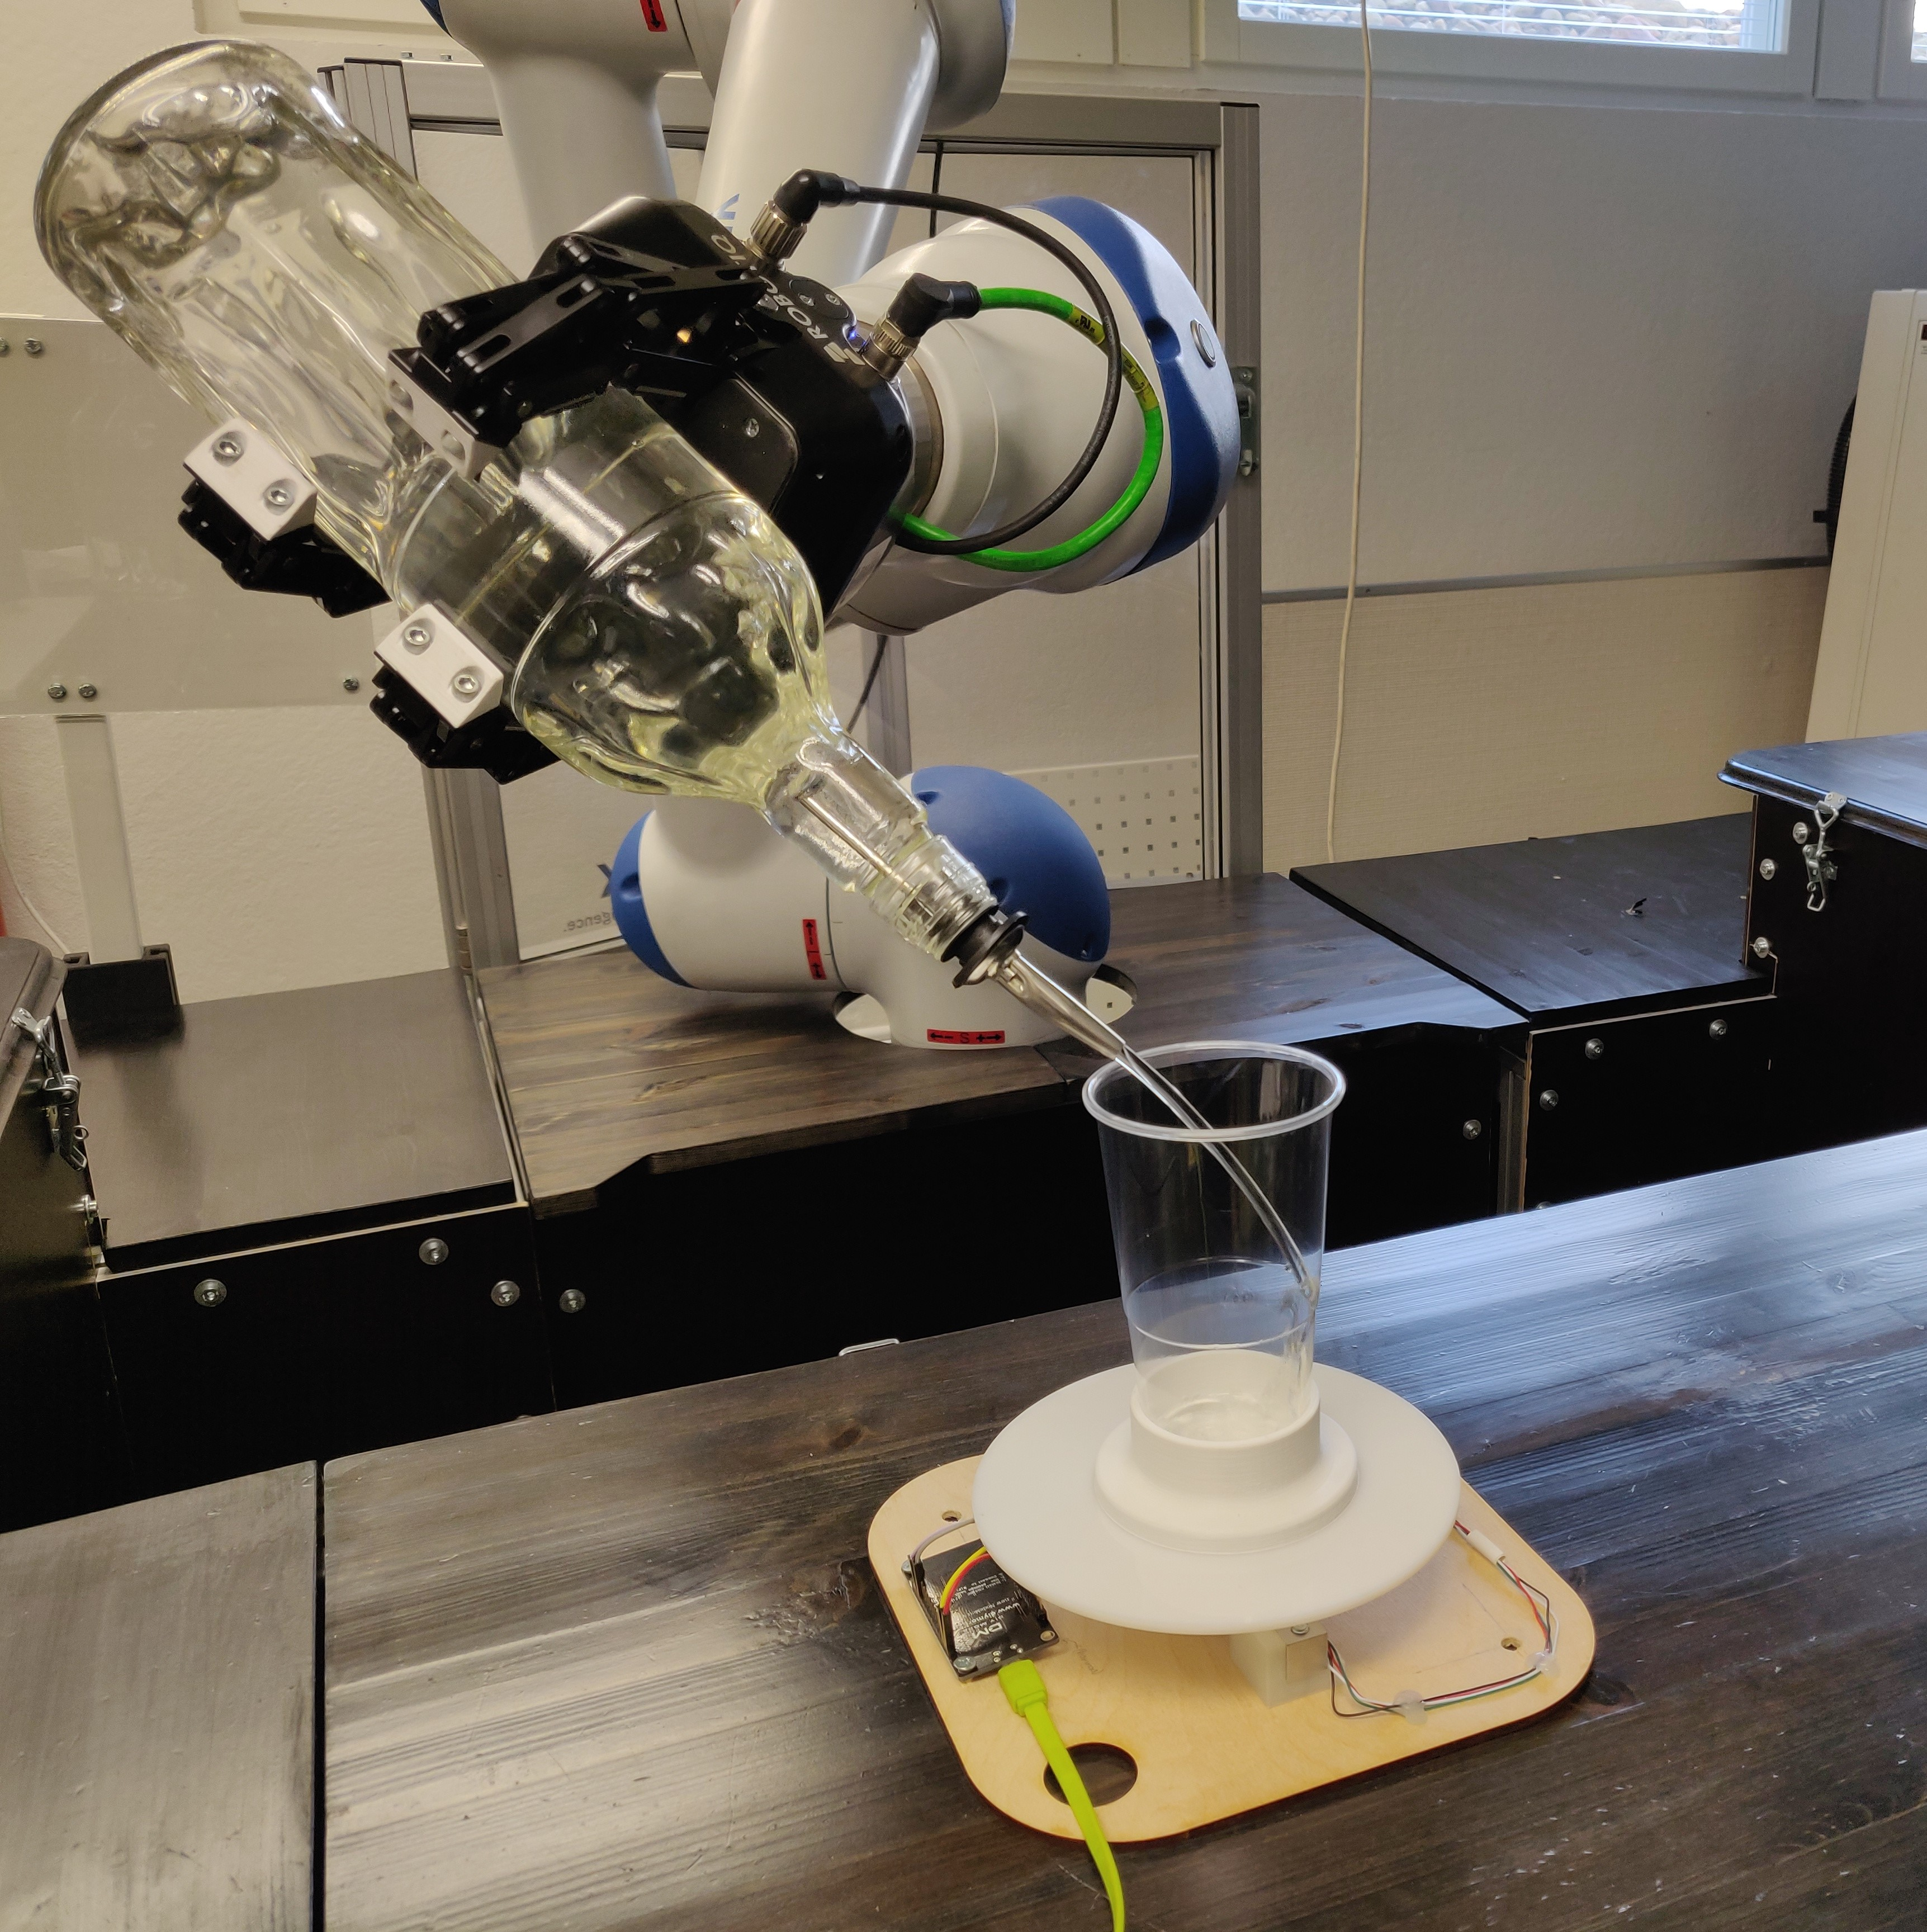
\includegraphics[scale=0.1]{img/kaato.jpg}
\end{center}
\caption{Robotti kaatoasennossa kaatamassa vaa'an päällä olevaan mukiin}
\label{fig:kaato}
\end{figure}

Uusi kaatosysteemi ei tällaisenaan mahdollista alle kolmen senttilitran kaatoja robotilla. Tämä johtuu siitä, että pelkkä kallistus- ja suoristusliikkeen aikana pullosta virtaava juoma on tilavuudeltaan noin kolme senttilitraa, vaikka robotti ei pysyisi kaatoasennossa paikallaan. Pienempiä kaatoja olisi luultavasti mahdollista saada muokkaamalla kaatoasennon kulmaa pienemmäksi. Alaluvussa \ref{ch:vanhan_ongelmat} luetellut lakisääteiset alkoholijuomien perusannokset eivät kuitenkaan vaadi alle neljän senttilitran kaatoja. Tämän takia pienten kaatojen mahdollisuutta ei lopulta ole tässäkään työssä toteutettu.
